% Created 2017-04-11 Tue 14:37
\documentclass[article,10pt]{article}
\usepackage[utf8]{inputenc}
\usepackage[T1]{fontenc}
\usepackage{fixltx2e}
\usepackage{graphicx}
\usepackage{longtable}
\usepackage{float}
\usepackage{wrapfig}
\usepackage{rotating}
\usepackage[normalem]{ulem}
\usepackage{amsmath}
\usepackage{textcomp}
\usepackage{marvosym}
\usepackage{wasysym}
\usepackage{amssymb}
\usepackage{hyperref}
\tolerance=1000
\date{April 11, 2017}
\title{Week 12 lecture notes - PSYC 5301}
\hypersetup{
  pdfkeywords={},
  pdfsubject={},
  pdfcreator={Emacs 25.1.1 (Org mode 8.2.10)}}
\begin{document}

\maketitle

\section*{Review discussion from Week 11}
\label{sec-1}

Last week, I asked each student to find an interesting result in the literature and compute a default Bayes factor (using JASP).  We discussed each of these examples from their discussion board in class.

\section*{Student presentations of their analyses of Lab 2 data}
\label{sec-2}

Also, I asked each student to begin playing with the Lab 2 data (arithmetic task) in JASP.  We discussed these preliminary analyses in class.

\section*{Review of factorial designs}
\label{sec-3}
\begin{itemize}
\item \emph{factors} - another name for independent variable
\begin{itemize}
\item ex: test mode
\end{itemize}
\item \emph{levels} - the values each factor can take
\begin{itemize}
\item ex: test mode has two levels: visual, auditory
\end{itemize}
\item an N x M factorial design has \emph{two} factors; the first with N levels and the second with M levels
\item Example: in our previous study, we had a 2 x 2 design.
\item Example: consider a 2 x 4 design:
\end{itemize}

\begin{center}
\begin{tabular}{lllll}
 & B1 & B2 & B3 & B4\\
\hline
A1 &  &  &  & \\
A2 &  &  &  & \\
\end{tabular}
\end{center}

The number of \emph{conditions} is calculated by multiplying the numbers of levels, so a 2x4 design has 8 conditions.

\subsection*{Anatomy of a 2x2 design}
\label{sec-3-1}

\begin{center}
\begin{tabular}{llll}
 & A1 & A2 & \\
\hline
B1 & condition mean A1B1 & condition mean A2B1 & marginal mean B1\\
B2 & condition mean A1B2 & condition mean A2B2 & marginal mean B2\\
\hline
 & marginal mean A1 & marginal mean A2 & \\
\end{tabular}
\end{center}

\begin{itemize}
\item if marginal means differ, this is called a \emph{main effect}
\item if pattern in one variable changes across the levels of the other, this is called an \emph{interaction}
\end{itemize}

\subsection*{Advantage of factorial design}
\label{sec-3-2}

If you have only one independent variable, there are only two possible outcomes: there is an effect, or there is not

If you have TWO independent variables, things are much more interesting!

Let 
\begin{itemize}
\item A = main effect of factor A
\item B = main effect of factor B
\item AB = interaction of A and B
\end{itemize}

Then there are EIGHT possible outcomes:
\begin{itemize}
\item No effects at all
\item A only
\item B only
\item AB only
\item A and B, but not AB
\item A and AB, but not B
\item B and AB, but not A
\item A, B, and AB
\end{itemize}

\subsection*{Examples of 2x2 designs}
\label{sec-3-3}

For each of the following:
\begin{itemize}
\item compute the marginal means
\item plot the means
\item decide whether the main effects and/or interactions are significant
\end{itemize}

\begin{center}
\begin{tabular}{lrr}
 & A1 & A2\\
\hline
B1 & 30 & 60\\
B2 & 30 & 60\\
\end{tabular}
\end{center}

\begin{center}
\begin{tabular}{lrr}
 & A1 & A2\\
\hline
B1 & 60 & 60\\
B2 & 30 & 30\\
\end{tabular}
\end{center}

\begin{center}
\begin{tabular}{lrr}
 & A1 & A2\\
\hline
B1 & 60 & 30\\
B2 & 30 & 60\\
\end{tabular}
\end{center}

\begin{center}
\begin{tabular}{lrr}
 & A1 & A2\\
\hline
B1 & 30 & 60\\
B2 & 30 & 30\\
\end{tabular}
\end{center}


\section*{Lab 2 manuscript assignment}
\label{sec-4}
\subsection*{Background}
\label{sec-4-1}
Independent variables:
\begin{itemize}
\item Problem size
\begin{itemize}
\item small: product less than or equal to 25
\item large: product greater than 25
\item within-subjects manipulation
\end{itemize}
\item Format
\begin{itemize}
\item digits
\item words
\item within-subjects manipulation
\end{itemize}
\end{itemize}

Dependent variables:
\begin{itemize}
\item number of problems completed (correctly)
\begin{itemize}
\item related to RT (as RT decreases, \# problems increases)
\end{itemize}
\item number of errors
\end{itemize}

Past research:
\begin{itemize}
\item problem size effect
\begin{itemize}
\item small problems faster than large problems
\item small problems less error prone than large problems
\end{itemize}
\item format effect
\begin{itemize}
\item digit problems faster than large problems
\item digit problems less error prone than large problems
\end{itemize}
\end{itemize}

The \emph{point} of our experiment is to examine whether problem size and format \textbf{interact}

Additive model of arithmetic (Dehaene and Cohen, 1995)

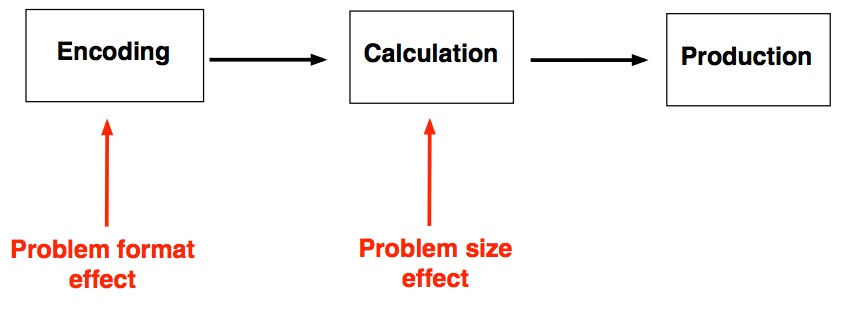
\includegraphics[width=.9\linewidth]{figures/dehaene1.jpg}

In this model, format effects are isolated only to encoding processes.

Interactive model of arithmetic (Campbell, 1999)

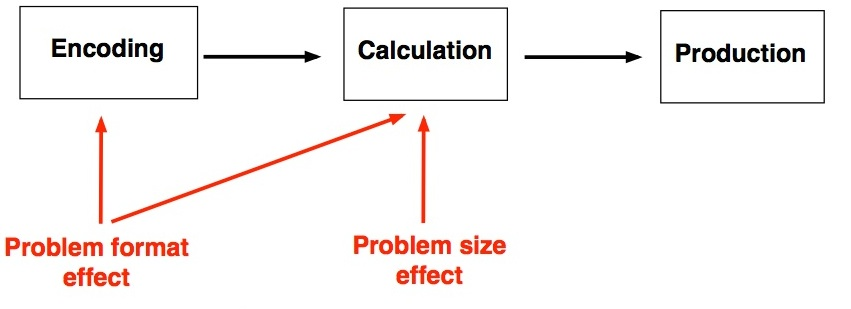
\includegraphics[width=.9\linewidth]{figures/campbell1.jpeg}

In this model, format affects both encoding AND calculation.

The critical test between these two models is whether there is a format x problem-size interaction!  This is completely testable in our experiment!  Your task is to test this prediction and arbitrate between these two competing models of mental arithmetic.

\section*{due dates:}
\label{sec-5}

IRB assignment: due Tuesday, April 25
Lab 2 manuscript: due Tuesday, May 9
% Emacs 25.1.1 (Org mode 8.2.10)
\end{document}